\chapter{Principal Component Analysis}
\label{chapter:pca}
\section{簡介}
\label{sec:background}


在機器學習中,資料的特徵(維度)數往往會影響模型的訓練效果,特徵太少可能所包含的資訊量太少,在進行模型訓練時,往往無法順利將資料進行正確的分類,所以會僅可能收集與資料集相關的特徵。但當資料的特徵多到一定的程度時,卻會因爲所包含的資訊太多,導致訓練出來的模型過擬合的現象,以至於分類器的效果不增反減,這種現象我們稱爲「curse of dimensionality」,如圖\ref{fig:curse_of_dimesionality}所示。所以在資料特徵過多的情況下,會進行資料降維,盡可能的減少模型發生過擬的現象,增加模型的訓練效果。

Principal Component Analysis(主成份分析),是一種非監督式的資料降維演算法,
主要是分析數據集中的一系列的主成份,將原本的數據集轉換到一個新的數據集。
其中在這一系列的主成份中,第一主成份,就是能在特徵空間中,找出一個投影向量,能使得這些資料的投影點能有最大的變異數,而第二主成份則是能找到第二大變異數的投影向量,以此類推。




\begin{figure}[h]
	\centering
	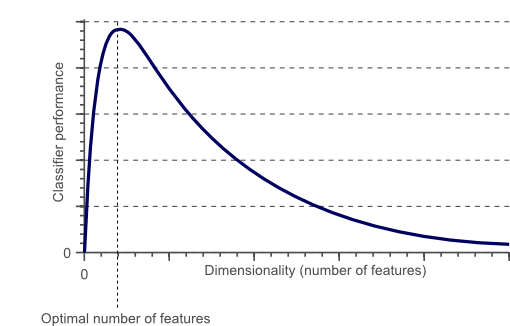
\includegraphics[height=5cm]{./pic/NZgacRXF.png}
	\caption{curse of dimensionality 示意圖}
	\label{fig:curse_of_dimesionality}
\end{figure}

\section{相關參數與實例說明}
為了更簡單理解這個演算法的數學義意,以下舉一個例子說明:

\subsection{相關參數}
\begin{itemize}
	\item
		\(\mathbf{x}\) 為原資料點, \(\overline{x}\) 表示原資料的均值。
	\item
	     \(\mathbf{z}\) 為過投影後資料點的值,\(\overline{z}\)則為投影後的均值。 
	\item
	      \(\mathbf{S}\) 資料變異量。而 \(\mathbf{{S}'}\)是資料經過投影後的變異量量。
	\item
	      \(v\) :投影向量。
\end{itemize}


\subsection{實例說明}

\begin{itemize}
	\item
	      圖\ref{fig:pca_demostrate}為一個具有兩個維度的資料分佈圖。


	      \begin{figure}[h]
		      \centering
		      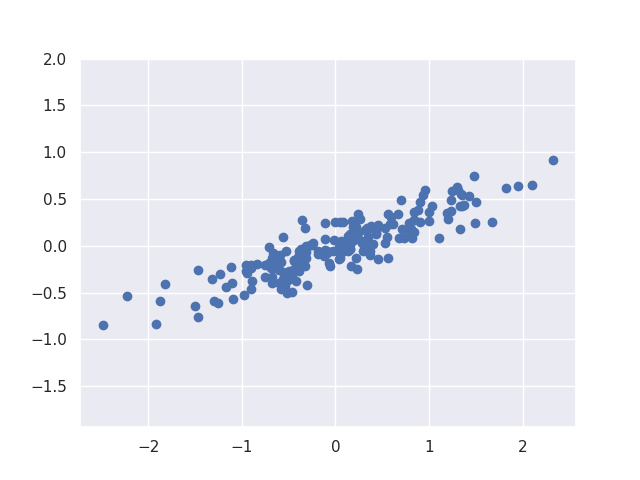
\includegraphics[width=9cm]{pic/pca_demostrate.png}
		      \caption{二維資料}
		      \label{fig:pca_demostrate}
	      \end{figure}


	      %
	\newpage
	\item
	      而PCA這個演算法的目的就是希望從這些資料點中如圖\ref{fig:pca_vector_to_find},找出投影向量,使得這些資料點投影在這些向量上後具有最大的變異數\footnote{\noindent 變異數:為對數據的變異程度的衡量,常用來量測資料分散程度之指標值,變異數其定義為 \(\sigma^2=\frac{{}\sum^{N}_{i}(x_i-\mu )^2}{N}\) }。
	      \begin{figure}[h]
		      \centering
		      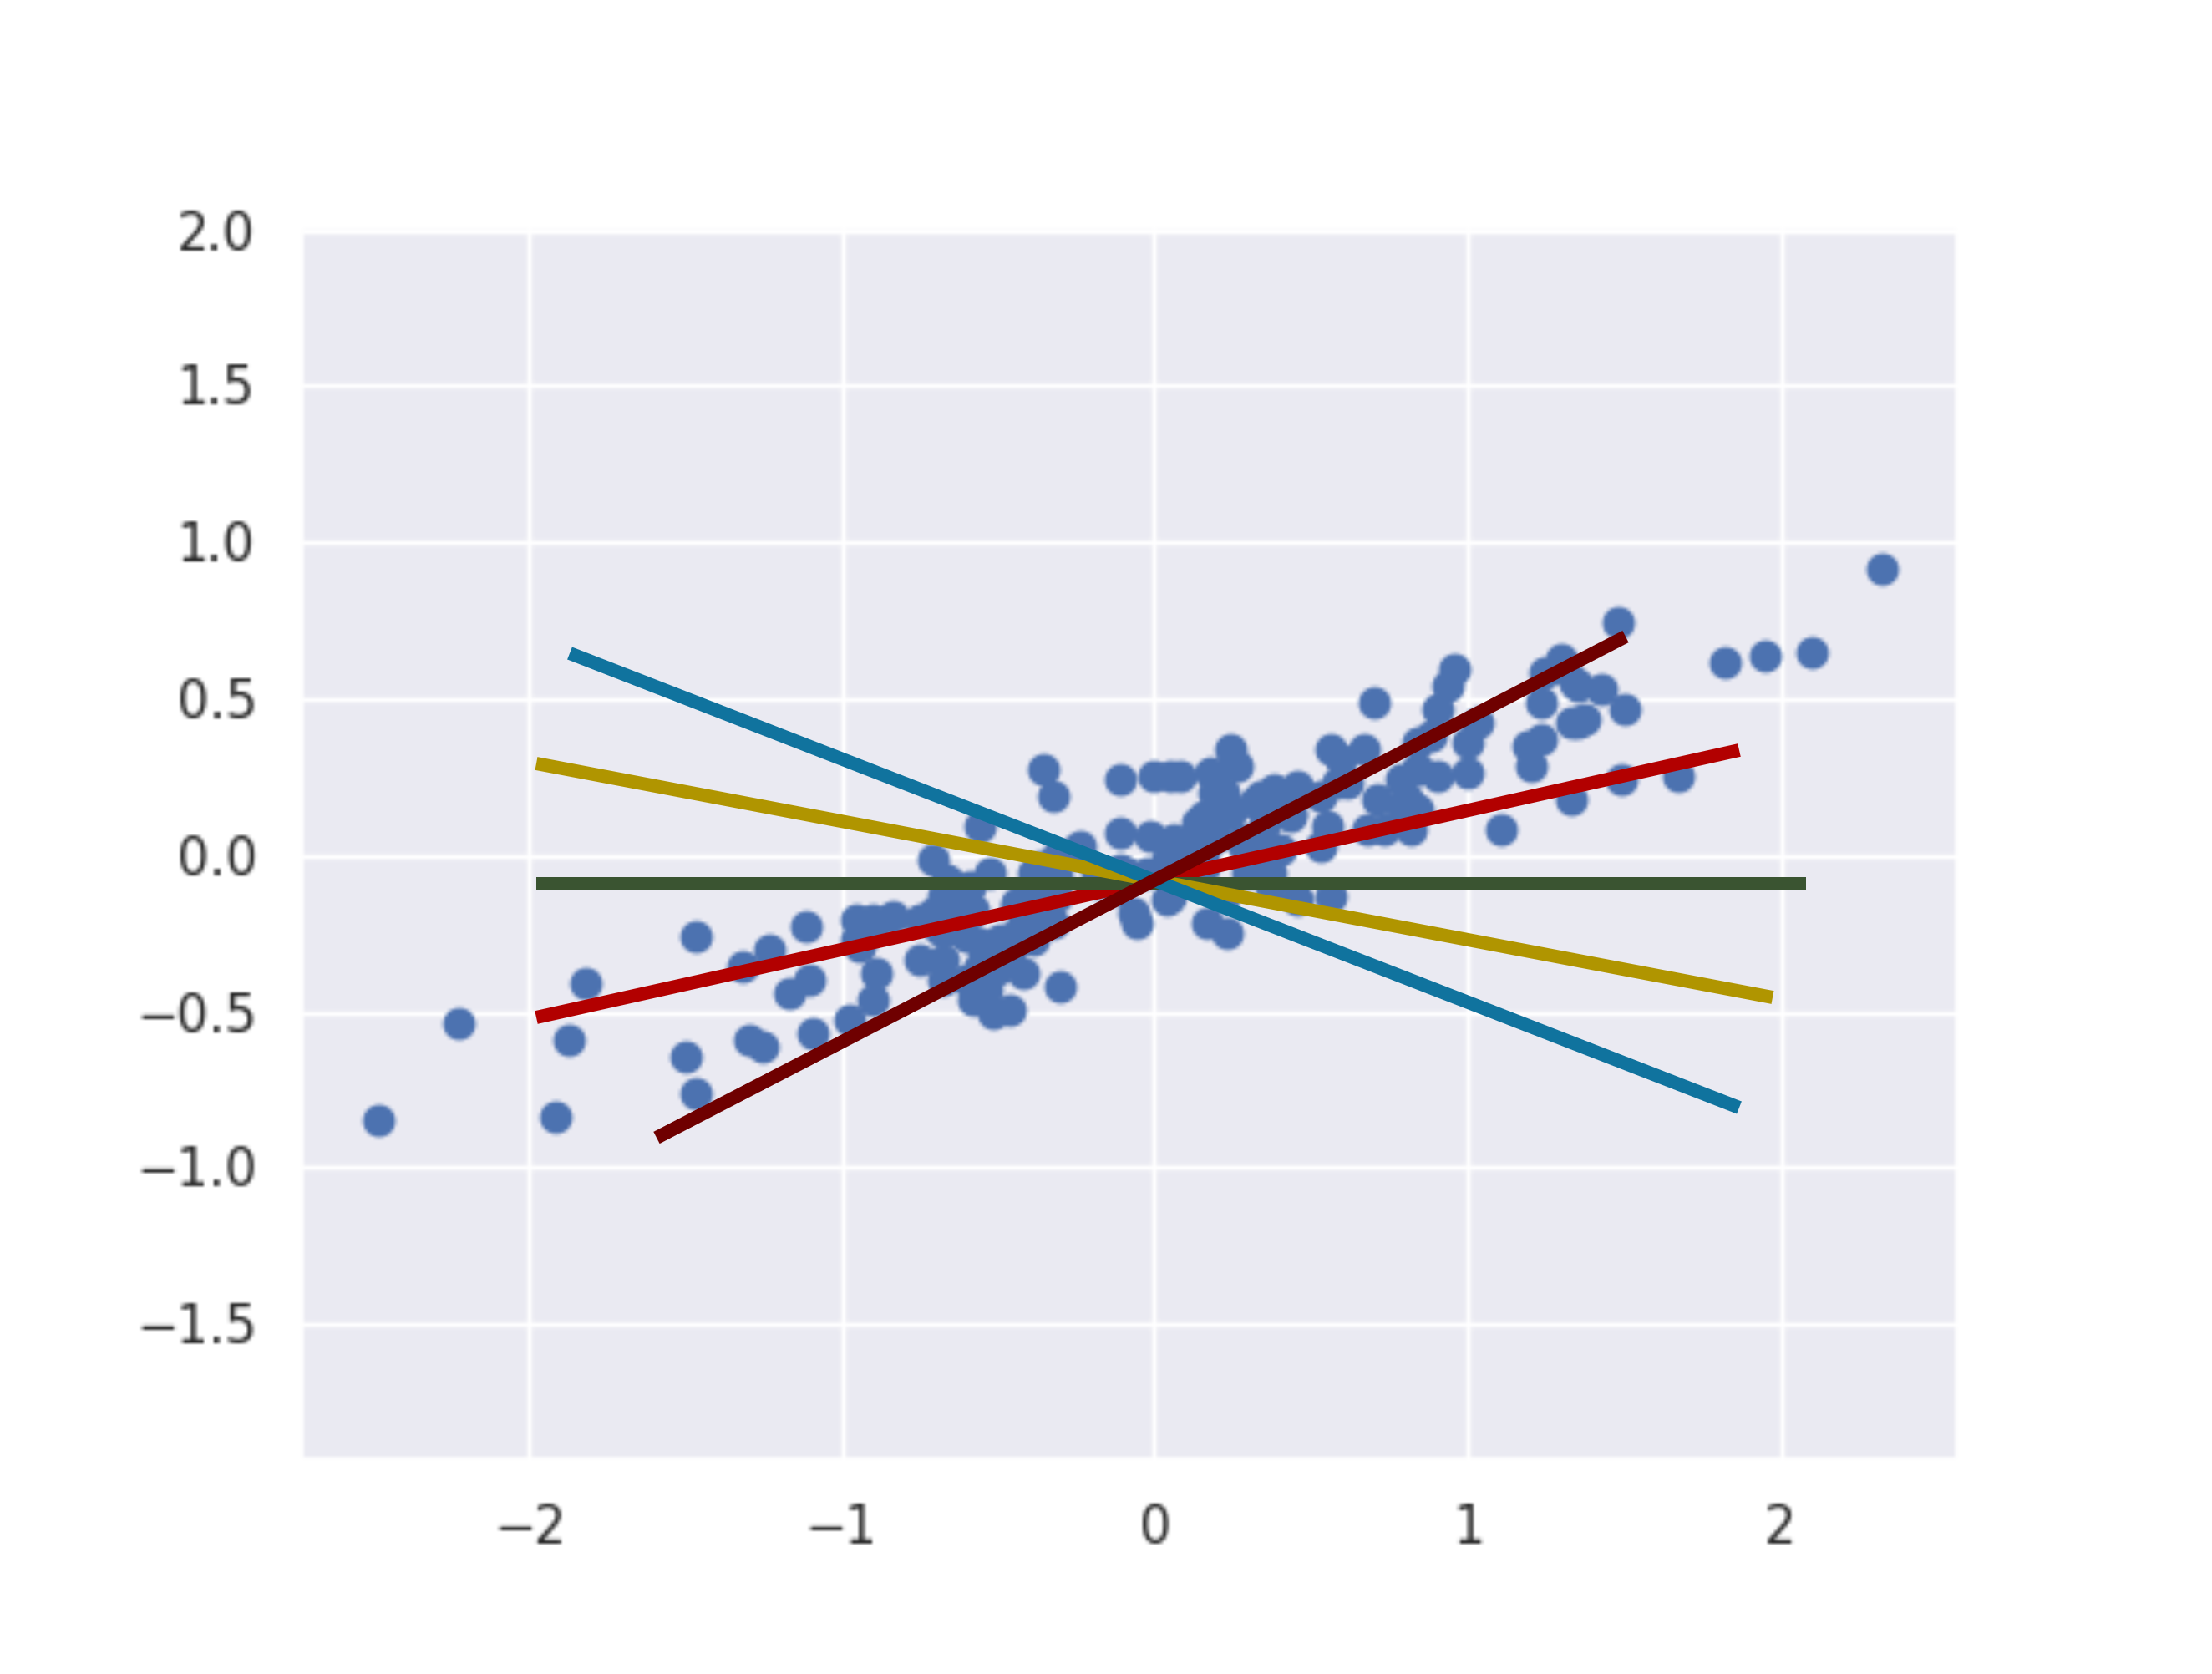
\includegraphics[width=9cm]{./pic/iVu9zQYG.png}
		      \caption{}
		      \label{fig:pca_vector_to_find}
	      \end{figure}
	      %
	\item
		式\ref{eqn:project_data}為投資料投影的公式,圖 \ref{fig:vector_project}為部分資料集於兩向量上的投影示意圖。 
		\begin{equation}
			\label{eqn:project_data}
			 z = vx
		\end{equation}


	      \begin{figure}[H]
		      \begin{center}
		      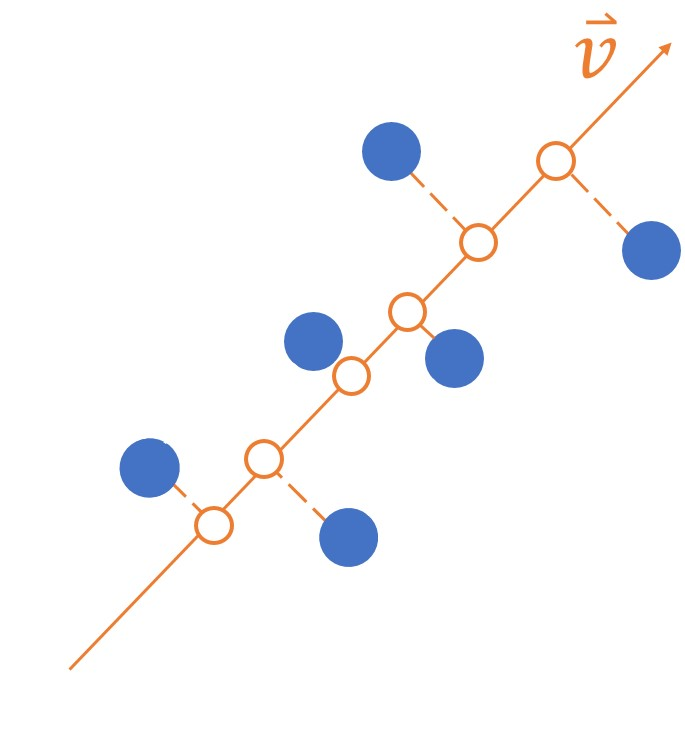
\includegraphics[width=5cm]{pic/pca_project_1.jpg}
			      \caption{部分資料集投影於向量上示意圖}
			      \label{fig:vector_project}
		      \end{center}
	      \end{figure}

	\item
		式\ref{eqn:variance_with_project}為資料進過投影後的變異量運算式。而圖 \ref{fig:pca_project_all}為部分資料集於兩向量上的投影示意圖,從圖 \ref{fig:pca_project_all}可以發現,資料於\(\vec{v}\)上的投影擁有較大的變異數。 

	      \begin{equation}
		      \label{eqn:variance}
		      \mathbf{S}  =\sum_{i=1} (x_i - \overline{x})(x_i-\overline{x})^T
	      \end{equation}

	      \begin{equation}
		      \label{eqn:variance_with_project}
		      \begin{aligned}
				  \mathbf{{S}'} &=\sum_{i=1} (z_i - \overline{z})(z_i-\overline{z})^T 
				  \\&=\sum_{i=1} (vx_i - v\overline{x})(vx_i-\overline{x})^T
				  \\&=v^T(\sum_{i=1} (x_i - w\overline{x})(x_i-\overline{x})^T)v
				  \\&=v^T\mathbf{S}v
		      \end{aligned}
	      \end{equation}



	      \begin{figure}[H]
		      \centering
		      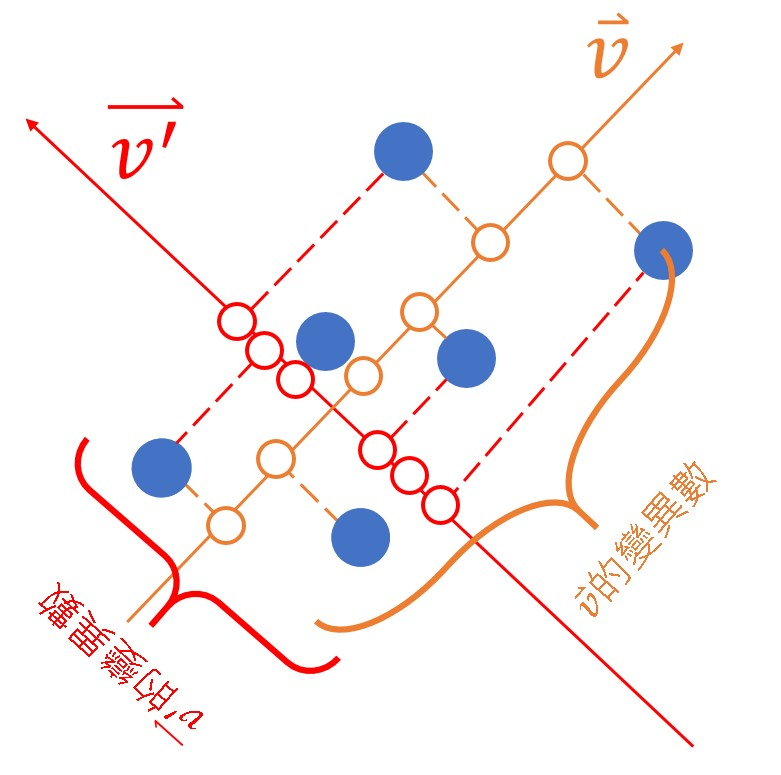
\includegraphics[width=6cm]{pic/pca_project_all.jpg}
			  \caption{\(\vec{v}\) 與\(\vec{{v}'}\)的變異數比較} 
		      \label{fig:pca_project_all}
	      \end{figure}
	      
	      %
	\item
		在PCA中,就是找出一個投影向量 \(v\) ,使得所有資料經過投影能有最大的變異數,如式\ref{eqn:max_projet_vector}。
		\begin{equation}
			\label{eqn:max_projet_vector}
			v = arg \underset{||v||_2=1}{max}\  v^TSv			
		\end{equation}


		\newpage
	\item
		經過PCA的計算之後,我們可以得到比較有代表性的兩個特徵成份,較長的為PC1,較短的為PC2,如圖\ref{fig:pc1_and_pc2}所示,而變異量的值分別為0.7625與0.0184 。


	      \begin{figure}[H]
		      \centering
		      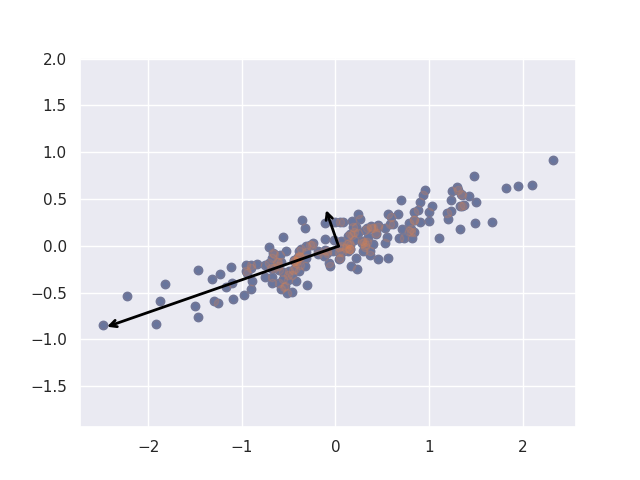
\includegraphics[width=9cm]{pic/pca_with_pca_axis.png}
		      \caption{}
		      \label{fig:pc1_and_pc2}
	      \end{figure}


	\item
	圖\ref{fig:pca_transform}為資料集經過PCA轉換的結果,橫軸為PC1,縱軸為PC2,能從圖中與上面得到的變異量發現,PC1所函概的資訊足以代表整個資料集。進而將原本二維的資料,轉換成一維,作為模型訓練的輸⼊。


	      \begin{figure}[H]
		      \centering
		      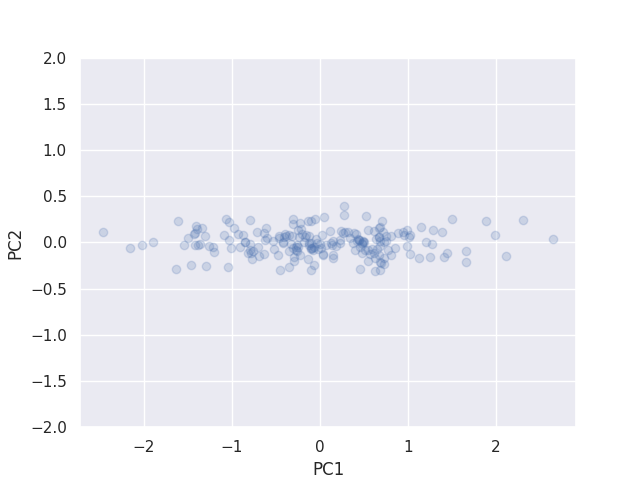
\includegraphics[width=9cm]{pic/pca_transform.png}
		      \caption{}
		      \label{fig:pca_transform}
	      \end{figure}

\end{itemize}


\section {結論}
從以上的舉例中,可以發現,經由PCA的轉換,我們可以分析出對於整個資料集最具代表性的成份,作為後序模型訓練的輸⼊資料。
也許二維的資料可能沒那麼明顯,但如果是影像資料(通常是具有高維度的資料),除了能夠有效的進行資料降維,提取影像中重要的特徵,還能因為維度的減少進而提高分類的運算速度。

